% Chapter 1

\chapter{Implementation} % Main chapter title

\label{Chapter 5} % For referencing the chapter elsewhere, use \ref{Chapter1} 

\lhead{Chapter 5. \emph{Implementation}} % This is for the header on each page - perhaps a shortened title
We described in previous chapters of the present thesis, the  problem  being addressed and our proposition for a solution. In the following, we present the implementation of this solution. 

\section{Development environment }
In order to implement the hybrid system Discolog, we used the  User Interface  DISCO \cite{rich2009building} as reactive HTN to which we integrate a prolog STRIPS planner to support the plan repair process. 

The most important challenge within the realization of such hybrid system is to support heterogeneous formalisms of Disco ans STRIPS. The system must be able to convert  the HTN domain knowledge from procedural formalizm implemented in Java to a declarative one capable to run in Prolog  and  handle exceptions related to this conversion. 

for that purpose, we integrated to DISCO the tuProlog  java-based light-weight Prolog engine to create a bridge that can use the logical prolog planner from the Java procedural environment . the environment architecture is described  in figure \ref{implementation environment of Discolog}.
	\begin{figure}[h]
		\centering
		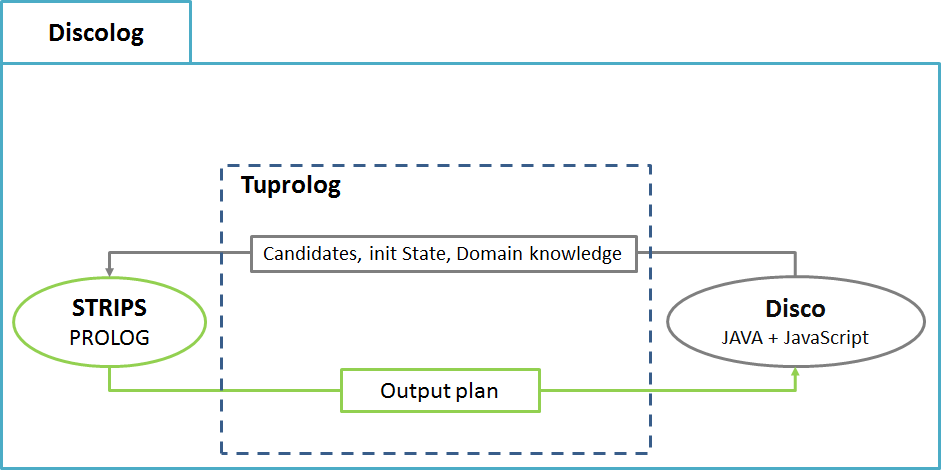
\includegraphics[width=250pt]{Pictures/archi1.png}
		\caption{\label{implementation environment of Discolog} implementation environment of Discolog}
	\end{figure}
	\section{DISCO}
 
 

DISCO \cite{rich2009building}is a task based user interface with a reactive architecture. The  most important feature of this reactive architecture is that allows the system to lead the user in a real time, without making any plan in advance. DISCO's functional architecture is composed by two mains components:
\begin{itemize}
	\item A \textit{task engine} whose function is to load and validate a task model description, and to maintain a representation	of the current status of the user’s tasks.\cite{rich2009building} In this present thesis, we only focus on this component. 
	\item \textit{User interface} to ensure the communication between the task engine and the user in the case where the engine needs more information or to help the user  achieving certain task.
	
	
\end{itemize}


%----------------------------------------------------------------------------------------
\subsection{DISCO task model}
Disco uses the ANSI/CEA-2018 standard for the procedural definition of the task model elements as described bellow :
\begin{itemize}
	\item \textit{Task}: The task model defines Task classes which are modeled using XML format.The figure \ref{xmldisco} describes eight task classes, including three compound tasks and  five primitive tasks. Primitive tasks may contain \textit{grounding script} parameter defined as JavaScript program which represent the effect of  the primitive task execution in the environment.

	\item \textit{Inputs and outputs} : Input includes all the data that may affect the execution of the task, and output includes all data that can be affected by the execution of the task. these data type is defined in JavaScript.
	\item \textit{Conditions} : Task's conditions (Preconditions, postconditions ans applicability conditions) are defined as boolean JavaScript function to evaluate the execution of a task.
			\begin{figure}[!h]
				\centering
				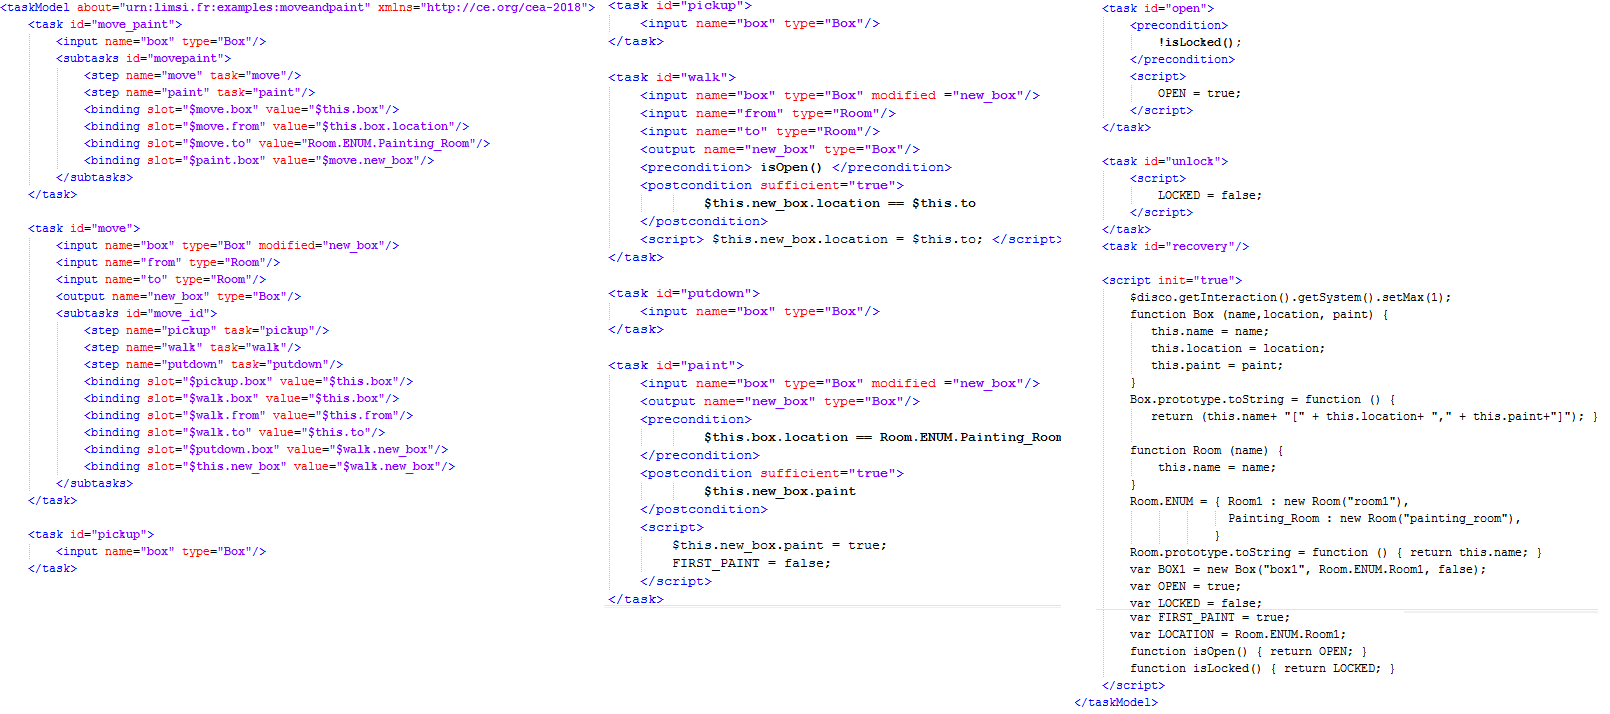
\includegraphics[width=\columnwidth]{Pictures/xmldisco.png}
				\caption{\label{xmldisco} Complete ANSI/CEA-2018 task model description for the moveandpaint task}
			\end{figure}
\end{itemize}
\section{Discolog implementation}
For the implementation of the Discolog system, we  faced some challenges. In addition to the management of heterogeneous environment, defining the level of information necessary to introduce in STRIPS domain knowledge required some reflection and designing a STRIPS planning algorithm able to provide effective solutions based on incomplete information in dynamic environment.
\subsection{The new Discolog API}
In order to implement the hybrid system Discolog we create the API shown in  figure \ref*{api} divided on two mains folders :
\subsubsection{Reactive DISCO }
We create an extension of DISCO that can detect breakdowns and in such case, collects a candidate list to the plan recovery process.In addition we manage to generate these candidates in the easiest way to be converted into PROLOG formalism. The input PROLOG planner is constituted in DISCO via TUprolog as demonstrated in the procedure input.
\lstinputlisting[language=Java]{Figures/input.java}

 Once the plan recover is generated, each action of this plan must be converted into primitive task formalism supported by DISCO. Therefore we create a procedure that treat and convert the STRIPS plan output as shown in the procedure output. 
\lstinputlisting[language=Java]{Figures/output.java}

\subsubsection{ Declarative PROLOG }
The main challenge faced in the creation of the STRIPS planner was to create an efficient means-end planning algorithm that can be integrated and executed  into TUprolog. Moreover, we had to define adequate structures that can receive the extracted domain knowledge  from the DISCO model using Tuprolog.Thus, we extract all the primitives tasks and turn them to a PROLOG formalism. 
 

		
		\begin{figure}[!h]
			\centering
			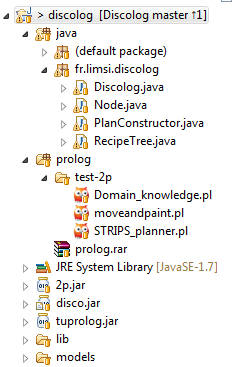
\includegraphics[width=.75\columnwidth]{Pictures/discologapi.png}
			\caption{\label{api} New structure of the Discolog API}
		\end{figure}
\section{Conclusion}

In this chapter, we described the implementation of the Discolog system. First we introduce the environment of the implementation and we introduced the DISCO system. Next we bring forward the new implemented Discolog API and explain each parts of this later.

in the next chapter, we present the experiments conducted to validate our system. 

% 
%\subsection{Description of the Discolog algorithm}
%%Let \textit{HTN} be a model of an Hierarchical Task Network with a top level task \textit{Goal} to achieve.To achieve \textit{Goal} Disco proceed as follow:
%%Starting from the top level goal \textit{Goal}, Disco recursively decomposes tasks until it reaches a set of primitives tasks that can achieve \textit{Goal}.
%%Each task in Disco has a \textit{status(Task)} $\in$ \{Live,Blocked,Done,Failed,Succeed\}.
%%\par Before decomposing a non primitive task or executing primitives task, Disco evaluate the precondition of the this task. If the current state holds the preconditions(Task) then status(Task) is updated to Live. otherwise, Status(Task)= Blocked and the HTN execution is blocked.
%%The same, after the execution of a primitive task(execution of the grounding script), Disco evaluate its postconditions. If postconditions(Task) are valid in the current state the status(Task) is updated to done or succeed, otherwise status(Task)= failed and the HTN execution become blocked.
%%
%%
%%At the end of the process, Disco(HTN,Goal) returns either Success(Goal is achieved) or failure if Disco faces breakdown. These breakdowns are detected if the top level goal is not achieved i.e Status(Goal) != Done and Disco has no decomposition or execution to propose. 
%%
%%When such breakdown occurs, Discolog invoke the Recover procedure which will first look over the \textit{Goal} and its children to find task candidates which can be repaired from the current state in order to recover from the breakdown. This process is handled by the procedure FindCandidates(), then call the STRIPS planner to propose a recover plan. \ref{euclid}. 
%\subsubsection{FindCandidate procedure}
%The procedure of finding  task candidates to be repaired checks every non executed task in the HTN affected by the breakdown. For each task, we extract the condition failed because of the breakdown: 
%\begin{itemize}
%	\item	If the status of task is neither done nor live then the algorithm will attempts to repair its preconditions
%	\item	If the status of task is failed then its postcondition are not valid and the repair algorithm will attempts to repair these postconditions.
%	\item	if the task is nonprimitive and all its applicability conditions are invalid in the current state then the algorithm will attempts te replan to satisfy one of its applicability condition. 
%\end{itemize}
%
%Once, the list of candidate is identified, it is then passed to the InvokeStrips procedure.
%\subsubsection{InvokeStrips procedure }
%	During this procedure, the planner will first constitute its initial state by observing the current state Next, for each candidate the mean-ends planner is called via TuProlog, and the best plan with the minimum cost is returned 
%	Finally, once the plan recovery is generated it has to be converted from prolog syntax to a procedural syntax supported by DISCO
	
	%----------------------------------------------------------------------------------------


%\begin{multicols}{2}
%\lstinputlisting[language=XML]{Chapters/moveandpaint.xml}
%\end{multicols}
%\lstinputlisting[language=XML]{Chapters/moveandpaint.xml}
